\documentclass[12pt,letterpaper]{article}
\usepackage{preamble}
\usepackage{tikzsymbols}
\usepackage{textcomp}
\usepackage{parskip}
%%%%%%%%%%%%%%%%%%%%%%%%%%%%%%%%%%%%%%%%%%
%%%% Edit These for yourself
%%%%%%%%%%%%%%%%%%%%%%%%%%%%%%%%%%%%%%%%%%
\newcommand\course{CSE 185}
\newcommand\hwnumber{1}

\newcommand\userID{Ramiro Gonzalez}

\begin{document}
\section{Must Know - Midterm I}
\begin{enumerate}
    \item Review Midterm 1 
\end{enumerate}
\section{Must Know - Midterm II}
\begin{enumerate}
    \item \textbf{ Derivative theorem of convolution}:  why do we want to compute $\frac{d}{dx}g$ (g is Gaussian filter) first and apply it to an image $f$ rather than convolve an image with g first and then take derivative of the image? Why can we do that? That is, why we can $\frac{d}{dx}(f*g) = f*\frac{d}{dx}g$\\
    \color{red}
 
    \begin{enumerate}
        \item Computing the derivative of the gaussian filter and then convolving the image $f$ saves us an extra step. \\
        \begin{tabular}{|c|c|}
        \hline
        \# 1 & Steps\\
        \hline
            f & "signal" function  \\
            $\frac{d}{dx}(g)$ & derivative of Gaussian (kernel)\\
            $f*\frac{d}{dx}(g)$ & Convolve with $\frac{d}{dx}(g)$ \\
            \hline
        \end{tabular}
        \begin{tabular}{|c|c|}
        \hline
            \#2 & Steps\\
            \hline
            f & "signal" function  \\
            g & kernel \\
            f*g & convolve image with g\\
            $\frac{d}{dx}(f*g)$ & take derivative of image\\
            \hline
        \end{tabular}
        
        \item Since differentiation is convolution, and convolution is associative then it holds that $\frac{d}{dx}(f*g) = f*\frac{d}{dx}g$, therefore we are allowed to do (\#1). 
    \end{enumerate}
    \color{black}
    \item \textbf{Image gradients}: how do we compute x  gradient and y gradient? how to compute the gradient direction? how to compute gradient magnitude?\\
    
    \color{red}
    \begin{enumerate}
        \item Sobel filter computes the gradients of input image. $I$ is the input image. 
        $$ H_y  =
    \begin{pmatrix}
    1 & 2 & 1\\
    0 & 0 & 0\\
    -1 & - 2 & -1 
    \end{pmatrix}$$
    $$ H_y  =
    \begin{pmatrix}
    1 & 0 & -1\\
    2 & 0 & -2\\
    1 & 0 & -1 
    \end{pmatrix}$$
        \begin{itemize}
            \item y gradient $G_y = H_y \circledast I$ (Horizontal edge response)
            \item x gradient $G_x = H_x \circledast I$ (Vertical edge response)
        \end{itemize}
        \item Compute gradient direction (orientation)
        $$\theta = \tan^{-1}(\frac{G_y}{G_x})$$
        \item Gradient magnitude 
        $$M = \sqrt{G_y^2 + G_x^2}$$
    \end{enumerate}
    %Use Derivative of Gaussian to compute image gradients 
    %begin{enumerate}
       % \item G: Gausssian function kernel. $I$ is the input image. 
       % \begin{itemize}
       %     \item x gradient $I_x = \frac{dG}{dx}\circledast I$
      %      \item y gradient $I_y = \frac{dG}{dy}\circledast I$
      %      
        %\end{itemize}
    %\end{enumerate}
    \color{black}
    \item \textbf{Canny edge detector}: how does non-maximum suppression work? how hysteresis process work?\\
    \color{red}
    \begin{enumerate}
        \item Non maximum suppression to is used to thin out the edges Non maximum suppression works by finding the pixel with the maximum value in an edge.
        \item For non-maximum suppression: At \textbf{q}, we have a maximum if the value is larger than those at both \textbf{p} and at \textbf{r}. Interpolate to get these values.
        \begin{center}
            \begin{figure}[h!]
                \centering
                \includegraphics[scale=0.5]{images/nonmax.png}
            \end{figure}
        \end{center}
        \item Hysteresis 
        \begin{itemize}
            \item Define two thresholds: low and high
            \item Use the high threshold to start edge curves and the low threshold to continue them.
        \end{itemize}
    \end{enumerate}
    \color{black}
    \item  What is Moravec detector? What is the problem with Moravec detector?\\
    \color{red}
    \begin{enumerate}
        \item Moravec detector is an corner detector
        \item It states that we should easily recognize the point by looking through a small window 
        \item Shifting a window in any direction should give a large change in intensity
        \item The problem with Moravec detector is as follows 
        \begin{itemize}
            \item Noisy response due to a binary window function
            \item Only a set of shifts at every 45 degree is considered
            \item Only minimum value of E is considered. 
        \end{itemize}
    \end{enumerate}
    \color{black}
    \item Harris corner detector: How does it work? What do the eigenvalues of the \textbf{M} matrix (i.e., second moment matrix based on image gradients) mean? Why do we measure cornerness using $R = \text{det}(M) - \alpha \text{trace}(M)^2$? How do you compute the determinant of M? How do you compute the trace of M?\\
    \color{red}
    $$M = \begin{bmatrix}
    \lambda_1 & 0 \\
    0 & \lambda_2
    \end{bmatrix}$$
    \begin{enumerate}
        \item Harris corner detection works as follows: 
        \begin{itemize}
            \item  Compute M matrix for each image window to get
their cornerness scores.
            \item Find points whose surrounding window gave large
corner response (f>threshold)
            \item Take the points of local maxima, i.e., perform non-
maximum suppression
        \end{itemize}
        \item The eigenvalues of the \textbf{M} matrix mean: 
        \begin{itemize}
            \item  If $\lambda_2 >> \lambda_1$ or  $\lambda_1 >> \lambda_2$  then it is an edge
            \item If $\lambda_1$ and $\lambda_2$ are large then the change of intensity \textit{E} increases in all directions therefore it is a corner. 
            \item If $\lambda_1$ and $\lambda_2$ are small (close to zero) then E (change of intensity) is constant in all directions. 
        \end{itemize}
        \item It is much simpler measure cornerness using $R$ than two values $\lambda_1, \lambda_2$ We measure cornerness using $R = \text{det}(M) - \alpha \text{trace}(M)^2$ because we find that if $R < 0$ then it is an edge and if $R > 0$ then it is a corner. If $|R|$ is small then it is a flat region. 
        \item M is a second moment matrix computed from image, 
        \begin{itemize}
            \item We compute the determinant as follows. Compute determinant of $2\times 2$ matrix $A =\begin{bmatrix}a & b \\ c & d\end{bmatrix} = ad - bc$
              $$M = \begin{bmatrix}
    \lambda_1 & 0 \\
    0 & \lambda_2
    \end{bmatrix} $$
            $$\text{det(M)} = \lambda_1\lambda_2$$
            \item We compute trace of M. Trace of matrix is $\text{trace(M)} = \sum_{i = 1}^{n} = m_{i,i}$ whhere (Just add diagonal values! \dSmiley)
      $$M = \begin{bmatrix}
    \lambda_1 & 0 \\
    0 & \lambda_2
    \end{bmatrix} $$
            $$\text{trace}{(M)} = \lambda_1 + \lambda_2$$
        \end{itemize}

    \end{enumerate}
    \color{black}
    \item What is Hough transform? When does it work well? When does it not?\\
    \color{red}
    \begin{enumerate}
        \item Hough transform is used for line fitting that is given a set of points it finds the curve or line that explains the data points best. Uses \textbf{Voting scheme}: For each feature point in the image, put a vote in every bin in the parameter space that could have generated this point
        \item It works well when: 
        \begin{itemize}
            \item Only works for a few parameters (1-4 typically)
        \end{itemize}
        \item It does not work well when: 
        \begin{itemize}
            \item When no prior pair match pair exist
            \item When there are many parameters
            \item There is a lot to noise (Noise = bad, +0.5 points)
            \item The grid size is bad. 
        \end{itemize}
    \end{enumerate}
    \color{black}
    \item What is RANSAC algorithm? How does it work?\\
    \color{red}
    \begin{itemize}
        \item \textbf{RANSAC( RANdom SAmple Consensus)} is used for line fitting it is a Learning technique to estimate
parameters of a model by random
sampling of observed data
        \item Algorithm (Repeat a-c until best model is found)
        \begin{enumerate}
            \item Sample (randomly) the number of points required to fit the model
            \item Solve for model parameters using samples
            \item Score by the fraction of inliers within a preset threshold of the model
        \end{enumerate}
    \end{itemize}
    \color{black}
    \item What is least squares line fitting? How does it work? What is the weakness of this method?\\
    \color{red}
    \begin{enumerate}
        \item Least squares line fitting is a \textbf{fitting and alignment} method that solves for translation
        \item It works as follows. 
        \begin{itemize}
            \item Write down objective funtion 
            \item Derived solution 
            \begin{itemize}
                \item Compute derivative 
                \item Compute solution 
            \end{itemize}
            \item Computational solution 
            \begin{itemize}
                \item Write in form $Ax = b$
                \item Solve using psudo-inverse or eigenvalue decomposition
            \end{itemize}
        \end{itemize}
        \item The weakness of this method is as follows: 
        \begin{itemize}
            \item It is not robust to outliers
        \end{itemize}
    \end{enumerate}
    \color{black}
    \item What is iterative closest point method? How/when do one method for model fitting?\\
    \color{red}
    \begin{enumerate}
        \item iterative closes point (ICP) is a fitting and alignment method.  It estimates transform between two dense sets of points
        \item Algorithm 
        \begin{enumerate}
            \item \textbf{Initialize} transformation (e.g., compute difference in means and scale
            \item \textbf{Assign} each point in \{Set 1\} to its nearest neighbor in \{Set 2\}
            \item \textbf{Estimate} transformation parameters - least squares or robust least squares 
            \item \textbf{Transform} the points in {Set 1} using estimated parameters
            \item Repeat steps i-iv until change is very small
        \end{enumerate}
        \item Local alignment only does not require initial correspondences 
    \end{enumerate}
    \color{black}
    \item \textbf{2D image transformations}: translation, Euclidean transform, similarity transform, affine transform, projective transform. How many parameters are there for each method? What are preserved for each transform?\\
    \color{red}
    \begin{figure}[h!]
        \centering
        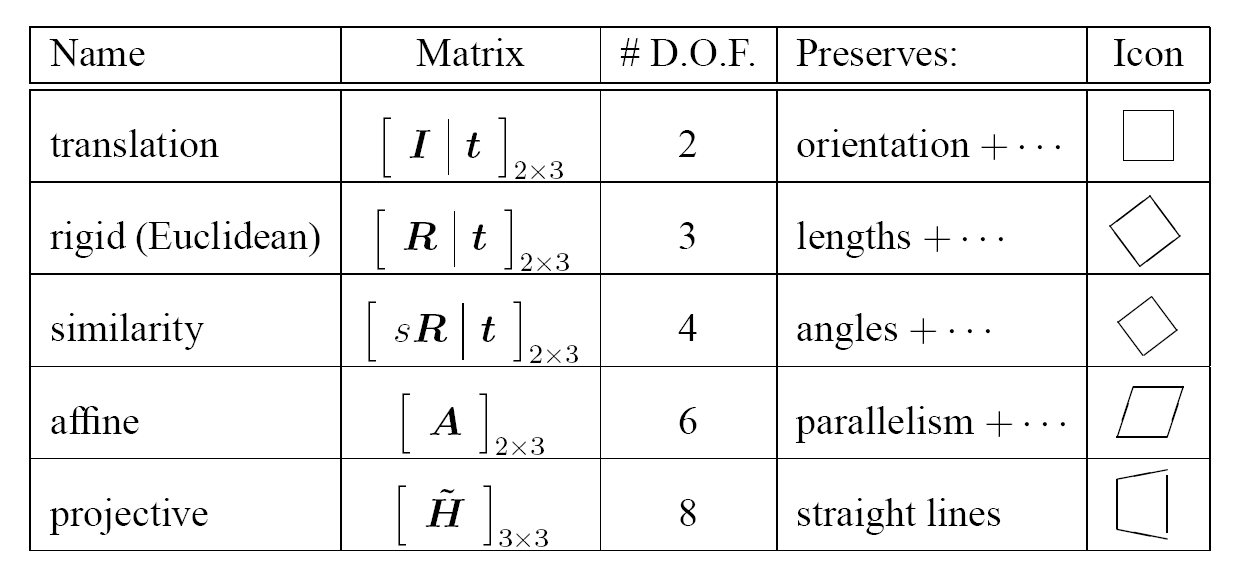
\includegraphics[scale=0.4]{images/transform.png}
    \end{figure}
    \begin{enumerate}
        \item Affine transformations are a combination of linear transformation and translations. 
    \end{enumerate}
    \color{black}
    \item \textbf{Geometry for a stereo system}. How do you derive the depth based on disparity?\\
    \color{red}
    \begin{figure}[h!]
        \centering
        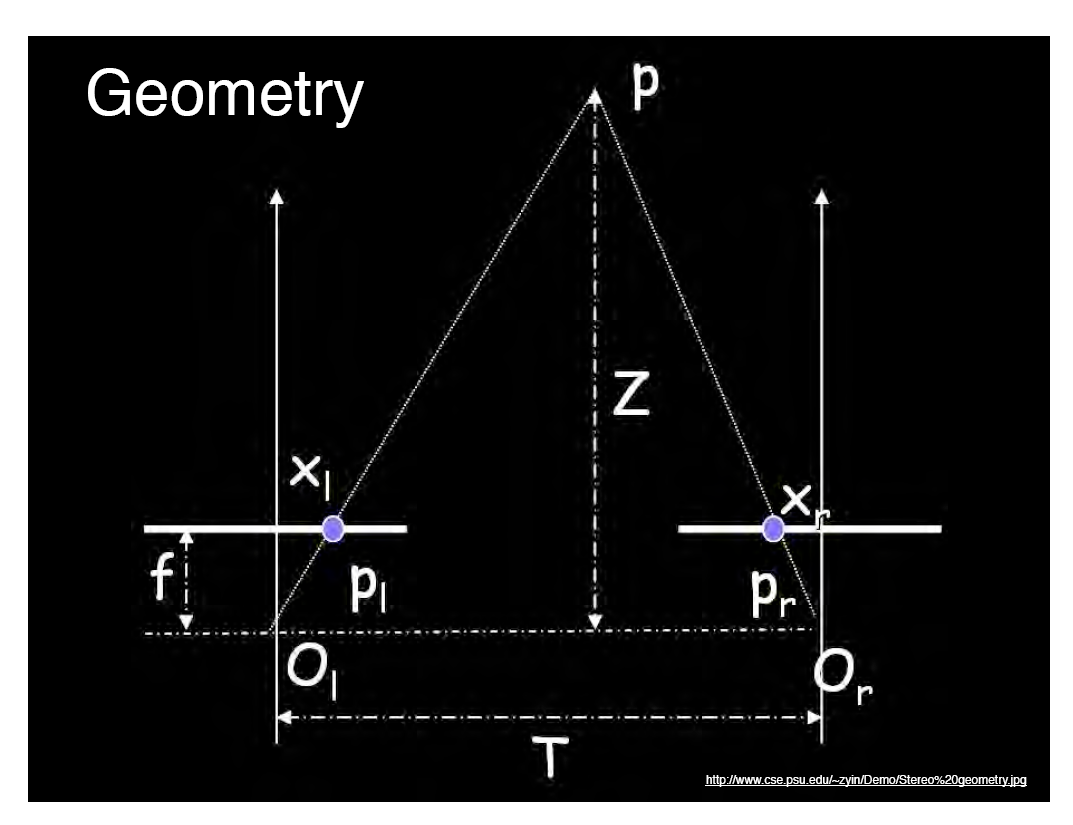
\includegraphics[scale=0.5]{images/geoStereo.png}
    \end{figure}
    \begin{enumerate}
        \item Assume parallel optical axes. (Calibrated cameras)
        \item Use similar triangles to derive depth based on disparity. 
        \item We know that there is triangle 1 $(p_1, P, p_r)$ and Triangle two: $(O_1, P, O_r)$
        $$\frac{T + (x_l - x_r)}{Z-f} = \frac{T}{Z}$$
        \item Disparity is $x_r - x_l$
)        $$Z = f(\frac{T}{x_r - x_1}$$
        \item  Depth from disparity: if we could find the corresponding points in two images, we could estimate relative depth
    \end{enumerate}
    \color{black}
    \item\textbf{ Epipolar geometry}: what is epipoles, how do you derive/compute the  epipolar line on the right image given one point on the left image? what do you use epipolar lines for?\\
    \begin{figure}[h!]
        \centering
        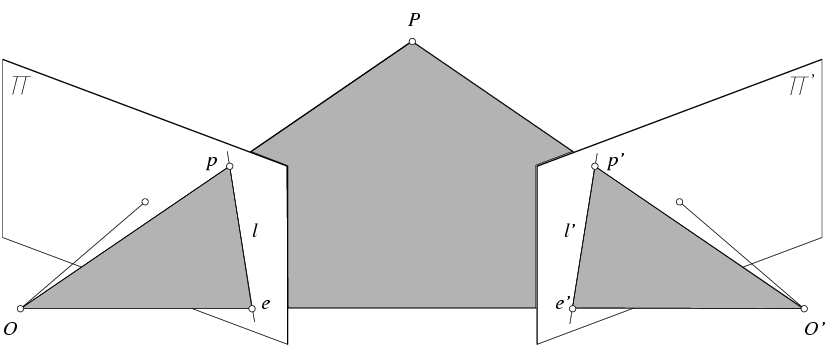
\includegraphics[scale=0.4]{images/test1.png}
        
    \end{figure}
    \color{red}
    \begin{enumerate}
        \item Epipole: point of intersection of baseline with image plane
        \item To derive/compute the epipolar line given on point on the left image we use the following formula\\
         An epipolar plane intersects the left and right image planes in epipolar lines\\
        Where $F$ is the fundamental matrix\\
       
        $$p'Fp = 0$$
        $$x'^{T}Fx = 0$$
        \item Epipolar line: intersection of epipolar plane with the image 
plane
    \end{enumerate}
    \color{black}
\end{enumerate}
\section{Problem Sets}
\subsection{Edge Detection}

\subsubsection{Canny Edge Detection and Laplacian-of-Gaaussian}
Compare the Canny edge detector and the Lapacian-of-Gaussian (LoG) edge detector for each of the following questions. 
\begin{enumerate}
    \item Which of these operators is/are isotropic and which is/are non-isotropic? \\
    \color{red}
    \textbf{Isotropic} operator in an image processing context is one which applies equally well in all directions in an image, with no particular sensitivity or bias towards one particular set of directions\\
    LoG is isotropic and Canny is non-isotropic
    \color{black}
    \item Describe each operator in terms of the order of the derivatives and that it computes.\\
    \color{red}
    LoG is second derivative and Canny is first derivative 
    \color{black}
    \item What parameters must be defined by the user of each operator? \\
    \color{red}
    LoG requires $\sigma$ defining the scale of the Gaussian blurring. Canny requires 
    $\sigma$ and two thresholds for hysteresis. 
    \color{black}
    \item Which detector is more likely to produce long, thin contours? Briefly explain. \\
    \color{red}
    Canny because of non-maximum suppression which thins and hysteresis thresholding which can fill in
    weak edge gaps. 
    \color{black}
\end{enumerate}
\subsubsection{Canny Edge Detection}
List   the   sequence   of   steps   involved   in   Canny   edge   detection,   including   image preprocessing. Describe the function of each step in one or two sentences.  \color{red}
\begin{enumerate}
    \item \textbf{Smoothing}:  Use  a  Gaussian  smoothing  filter  to  reduce  the  local  noise  in  the image. Edge detectors are strongly affected by noise, yielding many false positives. 
    \item \textbf{Computing gradients}: Use convolution filters(e.g., Sobel) to compute the vertical and horizontal components of the gradient throughout the image. This information will be used to estimate the strength and orientation of edges.
    \item \textbf{Assigning sectors}: Based on the orientation of local edges, assign each edge one of four orientation sectors. These will be used for non-maxima suppression. 
    \item \textbf{Non-maxima suppression}: Whichever pixel has a lower edge strength than either of  its  two  neighbors  in  the  direction  of  the  edge  gradient  (perpendicular  to  the  edge orientation) is set to zero. This way, detected edges are thinned to a width of one pixel.
    \item   \textbf{Hysteresis  thresholding}: Use  two edge  strength thresholds. Remove  any  pixel whose value is below the lower threshold, and pick as edge those pixels above the higher threshold. For  the  remaining  edge  candidates,  mark  them  as  edge  pixels  if  they  are connected  to  an edge  pixel  via  other  edge  candidates. This  final  step  will  remove  noise that is caused by small local variations in intensity that are not indicative of edges, and it will also fill gaps in contours.
\end{enumerate}
\color{black}
\subsection{True or False Questions}
\begin{enumerate}
    \item In Canny edge detector, non-maximum suppression is used to connect short edges. \\
    \color{red}
    FALSE.  Hysteresis threshold is used to connect short edges. Non maximum suppression is used to thin multi-pixel wide ridges down to single pixel width
    \color{black}
    \item Suppose $f(x)$ and $g(x)$ are two functions of x, so $\frac{d}{dx}(f*g) = f*(\frac{d}{dx}g)$, where * is the convolution operator. \\
    \color{red}
    TRUE: Differentiation is convolution, and convolution is associative 
    \color{black}
    \item If there is non-zero optical flow, it is always possible to infer something about the depth of
the scene shown in the image\\
    \color{red}
    FALSE: Apparent motion can be caused by lighting changes without any
actual motion
    \color{black}
    \item If we apply a Gaussian filter to an image and apply it again to the output, typically the image is smoothed more strongly than for a single application of the same filter.\\
    \color{red}
    TRUE: A Gaussian filter is a linear filter. It's usually used to blur the image or to reduce noise. If you use two of them and subtract, you can use them for "unsharp masking" (edge detection). The Gaussian filter alone will blur edges and reduce contrast.
    \color{black}
\end{enumerate}
\subsection{Multiple Choice Questions}
\begin{enumerate}
    \item Which of the following statements about Canny edge detector are true?
    \begin{enumerate}
        \item \color{red} The non-maximum suppression is used to select pixels that are close to true edges\color{black}
        \item \color{red}The edges found by Canny edge detector are determined by the Gaussian
kernel scale\color{black}
        \item In hysteresis process, we start with low thresholds and then high thresholds \\
        \color{blue}  In hysteresis process, we start with  high threshold and then low thresholds\color{black} 
        \item We can apply Gaussian filter to calculate the gradients of images\\
        \color{blue}We can apply Gaussian filter to calculate derivative of Gaussian filters or Sobel filters. \color{black}
    \end{enumerate}
    \item RANSAC. Which of the following statements are true when we use
RANSAC to fit data points with an objective function?
    \begin{enumerate}
        \item \color{red}RANSAC is robust to outliers \color{black}
        \item Not suitable for a large number of parameters
        \item \color{red}Optimization parameters are easier to choose than Hough transform \color{black}
        \item \color{red} Computational time grows quickly with fraction of outliers\color{black}
        \item Good for getting multiple fits
    \end{enumerate}
\end{enumerate}
\subsection{Assorted questions} 
\begin{enumerate}
    \item What is a difference between Gaussian smoothing and median filtering?
    How would you decide to use one vs another? \\
    \color{red}
    Median filter is more used for noise removal, more suitable for salt and pepper noise.
    Gaussian is used for smoothing and its better when noise not spiky. 
    \color{black}
    \item Under what conditions is the use of an affine transformation appropriate
    when viewing a planar scene?\\
    \color{red}
    If the field of view of the scene plane is such that all points visible on the world plane are at 
    approximately the same depth from the camera compared to the distance of the camera from the plane.
    \color{black}
    \item What effects can a planar affine transformation have on parallel lines?
    \\
    \color{red}
    Planar affine transformation preserve parallelism
    \color{black}
    \item In image processing, people usually apply Gaussian filter to images as pre-
processing step, before using the target filter, e.g. Sobel filter. Please give your
explanation to this Gaussian filtering operation. \\
\color{red}
        Gaussian filter is used to remove noise. 
\color{black}
\end{enumerate}
\section{Computational Questions}

\begin{enumerate}
    \item Hough transform. Given one point $(x,y) = (1,6)$ in the x-y plane, write down the corresponding line in the Hough 
    parameter space\\
    \color{red}
    Use the following: 
    $$y = mx + b$$
    $$\text{Haugh Space: } m = -\frac{1}{x}b + \frac{y}{x}$$
    $$m = -\frac{1}{x}b + \frac{y}{x} = -b + 6$$
    \color{black}
\end{enumerate}
\subsection{Harris Corner}
Here is the second moment matrix for Harris corner detection. 
$$\sum_{x,y} w(x,y)\begin{bmatrix}I_{x}^{2} & I_xI_y\\ I_xI_y & I_{y}^2\end{bmatrix}$$
When evaluated at 3 patches A, B, C of an image, the eigenvalues of the matrices are 
$$A: \lambda_1 = 0.9, \lambda_2 = 0.01; B: \lambda_1 = 0.012, \lambda_2 = 0.014; C: \lambda_1 = 0.9, \lambda_2 = 0.92$$
\begin{center}
\begin{figure}[h!]
    \centering
    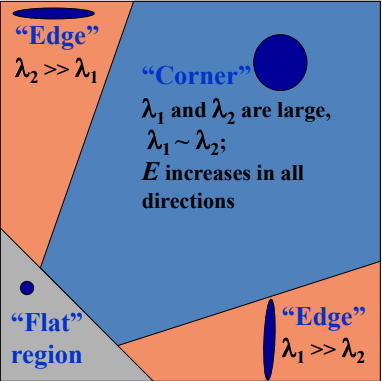
\includegraphics[scale=0.5]{images/ecf.png}
\end{figure}
\end{center}
If we know that amount A, B, C, there is a corner, an edge, and a flat region. What are A,B,C respectively? Fill in the balnks below with A,B,C. \\
Flat Region: \color{red} B \color{black}\\
Corner: \color{red} C \color{black} \\
Edge: \color{red} A \color{black}
\\
\textbf{Review Midterm II}
\section{New Material}
\begin{enumerate}
    \item Optical flow: what are the assumptions? how do you estimate the optical flow using  the Lucas-Kande algorithm? How do the eigenvalues in the covariance matrix relate to Harris corner detector? \\
    \color{red}
    \begin{enumerate}
        \item Optical flow is an approximation of the motion field
        \item Assume the image intensity  I  is constant
        \item Estimate velocity at each pixel using one iteration of Lucas and Kanade estimation
        \item 
    \end{enumerate}
    \color{black}
    \item  Eigenface problems: what is PCA? what is a covariance matrix? why are the top eigenvectors important? what do they describe the data distribution?
    \item Clustering methods: when does the K-means clustering method perform well? what are the pros and cons of the K-means clustering method? Likewise, what are the pros and cons of the agglomerative clustering method?
\end{enumerate}
\end{document}
  
    .
